\documentclass[border=1.5pt]{standalone}
\usepackage{amsmath,amssymb}
\usepackage{tikz}
\usetikzlibrary{arrows.meta,calc,positioning,shapes,shapes.misc,shapes.geometric,backgrounds,fit,decorations.pathreplacing,quantikz2}
% Shared colors and styles for the XYZ^2 figures.
% Pauli types: bright tones for fills and bands, deep (800) shades of the same hues for labels.
% The label shades keep the hue of each Pauli, are well separated from each other (CIEDE2000 > 20)
% and have a contrast ratio of at least 2.9 on the coral cells and 4.5 on the sunflower cells.
\definecolor{PauliX}{HTML}{F97316}
\definecolor{PauliY}{HTML}{EC4899}
\definecolor{PauliZ}{HTML}{9333EA}
\definecolor{PauliXText}{HTML}{AC340B}
\definecolor{PauliYText}{HTML}{9D174D}
\definecolor{PauliZText}{HTML}{5B21B6}
% Generator classes: S0 (class B, even links, coral) and gauge (class A, odd links, sunflower)
\definecolor{Szero}{HTML}{F0435E}
\definecolor{SzeroText}{HTML}{BE123C}
\definecolor{Gauge}{HTML}{F59E0B}
\definecolor{GaugeText}{HTML}{B45309}
\colorlet{GaugeGray}{Gauge}
\definecolor{ClassB}{HTML}{FF8A99}
\definecolor{ClassA}{HTML}{FFD23F}
% Logical operators (X-bar violet, Z-bar crimson), errors, ink
\definecolor{LogicalZ}{HTML}{E11D48}
\definecolor{LogicalGold}{HTML}{7C3AED}
\definecolor{ErrRed}{HTML}{1C1917}
\definecolor{InkDark}{HTML}{292524}
\definecolor{InkSoft}{HTML}{57534E}
% Labels drawn on top of colored cells
\colorlet{CellText}{InkDark}
% Noise channels
\definecolor{ErrFlip}{HTML}{EF4444}
\definecolor{Idle}{HTML}{EC4899}
\definecolor{TwoQ}{HTML}{7C3AED}
% Protocol steps
\definecolor{StepPrep}{HTML}{F97316}
\definecolor{StepMeas}{HTML}{D946EF}
\definecolor{StepDec}{HTML}{7C3AED}
\definecolor{StepRec}{HTML}{DB2777}
\tikzset{
  qb/.style={circle, draw=InkDark, line width=0.6pt, fill=white,
             minimum size=4.2mm, inner sep=0pt, font=\scriptsize},
  qbsmall/.style={circle, draw=InkDark, line width=0.5pt, fill=white,
             minimum size=2.6mm, inner sep=0pt},
  hexedge/.style={line width=0.65pt, draw=InkSoft},
  linkedge/.style={line width=1.6pt, draw=InkDark},
  bndedge/.style={line width=0.65pt, draw=InkSoft, densely dashed},
  plabel/.style={font=\scriptsize\bfseries, inner sep=1pt},
  panel/.style={font=\small\bfseries, anchor=north west},
}

\providecommand{\ket}[1]{\left|#1\right\rangle}

\begin{document}
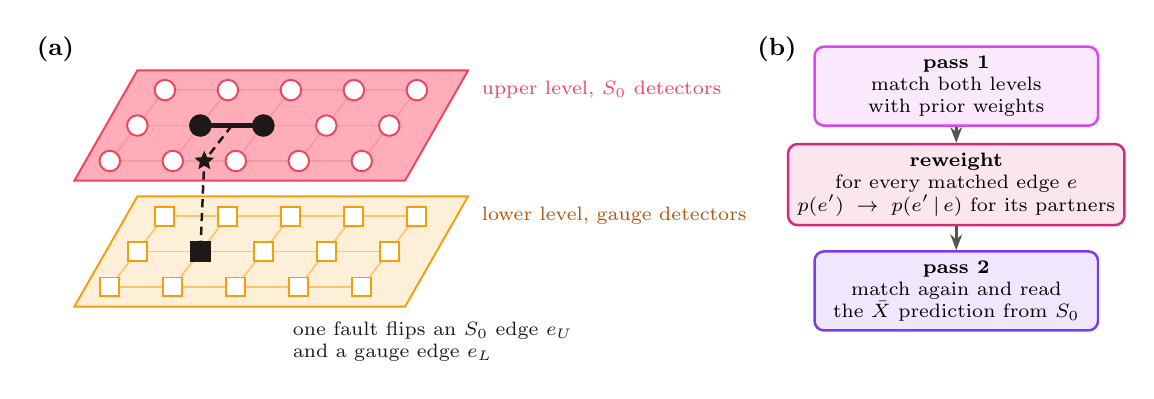
\begin{tikzpicture}[
  udet/.style={circle, draw=Szero, line width=0.7pt, fill=white, minimum size=2.6mm, inner sep=0pt},
  ldet/.style={rectangle, draw=Gauge, line width=0.7pt, fill=white, minimum size=2.4mm, inner sep=0pt},
  hot/.style={fill=ErrRed, draw=ErrRed},
  uedge/.style={line width=0.6pt, draw=Szero!55},
  ledge/.style={line width=0.6pt, draw=Gauge!60},
  step/.style={draw=#1, fill=#1!12, line width=0.9pt, rounded corners=1.2mm, font=\scriptsize, align=center, minimum width=3.6cm},
]
% ===================== panel (a): two levels of the detector graph
\begin{scope}[shift={(0,0)}]
  \node[panel] at (-0.6,3.55) {(a)};
  % upper plane (S0)
  \draw[fill=ClassB!70, draw=Szero, line width=0.7pt] (0,1.6) -- (4.2,1.6) -- (5.0,3.0) -- (0.8,3.0) -- cycle;
  \node[font=\scriptsize, text=Szero, anchor=west] at (5.05,2.75) {upper level, $S_0$ detectors};
  % lower plane (gauge)
  \draw[fill=Gauge!16, draw=Gauge, line width=0.7pt] (0,0) -- (4.2,0) -- (5.0,1.4) -- (0.8,1.4) -- cycle;
  \node[font=\scriptsize, text=GaugeText, anchor=west] at (5.05,1.15) {lower level, gauge detectors};
  % grids
  \foreach \i in {0,...,4}{
    \foreach \j in {0,...,2}{
      \pgfmathsetmacro{\x}{0.45+0.8*\i+0.35*\j}
      \pgfmathsetmacro{\y}{1.85+0.45*\j}
      \pgfmathsetmacro{\yl}{0.25+0.45*\j}
      \coordinate (U\i\j) at (\x,\y);
      \coordinate (L\i\j) at (\x,\yl);
    }
  }
  \foreach \i in {0,...,3}{\foreach \j in {0,...,2}{
    \pgfmathtruncatemacro{\ii}{\i+1}
    \draw[uedge] (U\i\j) -- (U\ii\j); \draw[ledge] (L\i\j) -- (L\ii\j);}}
  \foreach \i in {0,...,4}{\foreach \j in {0,...,1}{
    \pgfmathtruncatemacro{\jj}{\j+1}
    \draw[uedge] (U\i\j) -- (U\i\jj); \draw[ledge] (L\i\j) -- (L\i\jj);}}
  \foreach \i in {0,...,4}{\foreach \j in {0,...,2}{
    \node[udet] at (U\i\j) {}; \node[ldet] at (L\i\j) {};}}
  % fault: one gauge detector + two S0 detectors
  \node[udet, hot] at (U11) {}; \node[udet, hot] at (U21) {};
  \node[ldet, hot] at (L11) {};
  \draw[line width=1.6pt, draw=ErrRed] (U11) -- (U21);
  % the fault sits in the gap between two detectors of the lowest row
  \coordinate (F) at ($(U10)!0.5!(U20)$);
  \draw[densely dashed, line width=0.9pt, draw=ErrRed] ($(U11)!0.5!(U21)$) -- (F) -- (L11);
  \node[star, star points=5, star point ratio=2.2, fill=ErrRed, minimum size=2.6mm, inner sep=0pt] at (F) {};
  \node[font=\scriptsize, text=ErrRed, anchor=west, align=left] at (2.65,-0.45) {one fault flips an $S_0$ edge $e_U$\\ and a gauge edge $e_L$};
\end{scope}
% ===================== panel (b): two passes
\begin{scope}[shift={(9.3,0.2)}]
  \node[panel] at (-0.75,3.35) {(b)};
  \node[step=StepMeas] (p1) at (1.9,2.6)
     {\textbf{pass 1}\\ match both levels\\ with prior weights};
  \node[step=StepRec] (rw) at (1.9,1.35)
     {\textbf{reweight}\\ for every matched edge $e$\\ $p(e')\;\to\;p(e'\,|\,e)$ for its partners};
  \node[step=StepDec] (p2) at (1.9,0.0)
     {\textbf{pass 2}\\ match again and read\\ the $\bar X$ prediction from $S_0$};
  \draw[-{Stealth[length=2mm]}, line width=0.9pt, draw=InkSoft] (p1) -- (rw);
  \draw[-{Stealth[length=2mm]}, line width=0.9pt, draw=InkSoft] (rw) -- (p2);
\end{scope}
\end{tikzpicture}

\end{document}
